\chapter{Bevezetés}
Ebben a dolgozatban a BME VIK Villamosmérnök MSc képzés Önálló Laboratórium 1 c. tárgyának keretében végzett kutatási és tervezési munkámat összegzem. A dolgozatom témája egy kevéssé ismert nyomtatott antennatípus, a BIFA (Balanced Inverted F Antenna) tervezése.
\section{Antennák jellemzői}
	A különböző antennák összehasonlításának jó eszközei a következő paraméterek, amelyek segítségével több szempontból nyerhetünk betekintést az antennák működésébe.
\par A számszerűsíthető antennaparaméterek kifejtése előtt megemlítem a reciprocitási tételt, ami szerint egy antennát adóantennaként vizsgálva ugyanazokat a paramétereket kapjuk, mint vevő üzemmódban, emiatt elég csak az egyik esetet vizsgálni a kettő közül és az eredmények érvényben maradnak a másik esetben is, csak az energia áramlásának iránya fordul meg a szabad tér és az antenna között.
	\subsection{Iránykarakterisztika, irányhatás és nyereség}
		\par Az antennák alapvető célja, hogy messzire jutó elektromágneses hullámokat hozzanak létre. A létrehozott hullámok energiát szállítanak, teljesítmény áramlik belőlük a szabad térbe. A sugárzási tulajdonságok leírásához gömbi koordinátarendszert $(r, \theta, \phi)$ szokás használni. Az antenna (teljesítmény-) iránykarakterisztikája ($G(\theta, \phi)$) azt írja le, hogy egy az antenna körüli, megfelelően nagy $r$ sugarú gömb felületén hogyan oszlik el az antenna bemenetén betáplált teljesítmény. A nyereség képlete \aref{equ:G}. egyenletben látható, ahol $S(r,\theta,\phi)$ a gömbi koordinátákkal megadott pontban az antenna által létrehozott felületi teljesítménysűrűség, $P_{be}$ az antennába betáplált teljesítmény, $S_0$ pedig az ideális izotróp antenna által létrehozott felületi teljesítménysűrűség azonos $r$ távolságban.
		\begin{align}
			\begin{split}
				\label{equ:G}
				G(\theta,\phi) & = \frac{S(r,\theta,\phi)}{S_0}\\
				S_0 & = \frac{P_{be}}{4\pi r^2}
			\end{split}
		\end{align}
		\par Az iránykarakterisztika értéke egy adott $(\theta, \phi)$ irányban, az ahhoz az irányhoz tartozó nyereség. A szakirodalomban a nyereség kifejezés alatt legtöbbször az iránykarakterisztika maximumát kell érteni, ezt hol $G_{max}$-szal, hol egyszerűen $G$-vel jelölik ezt és általában nem viszonyszámban, hanem dB-ben adják meg. A továbbiakban $G$-vel jelölöm a nyereség dB-ben kifejezett értékét.
		\par Az irányhatás a nyereséghez nagyon hasonló mennyiség, a kettő között az egyedüli különbség, hogy a nevezőben szereplő $P_{be}$ összes betáplált teljesítmény helyett az irányhatás esetében $P_{s}$ összes kisugárzott teljesítmény szerepel.
		\begin{align}
			\begin{split}\label{equ:D}
				D & = \frac{S(r,\theta,\phi)}{S_0'}\\
				S_0' & = \frac{P_s}{4\pi r^2}
			\end{split}
		\end{align}
		\par Ez azt jelenti, hogy a nyereségnél figyelembe vesszük az antenna veszteségeit, míg az irányhatásnál nem.
\section{Monopól antennák}
\par A BIFA antennatípus nem gyakori a szakirodalomban, az irodalomkutatás során csak a Silicon Laboratories egy 2014-es application note-jában \cite{an847} találkoztam vele \huge{ÉS MÉG MÁSHOL IS MERT NEM BACK HANEM BALANCED}. \normalsize Ez az antennatípus egy variációja az IFA-nak (Inverted F Antenna, \aref{fig:tipikus_ifa}. ábra), ezért az IFA jellegzetességeiből kiindulva érdemes tárgyalni, amihez érdemes megvizsgálni a monopól antennák általános jellemzőit, mivel az IFA is ebbe az antennacsaládba tartozik.
\begin{figure}[h]
	\centering
	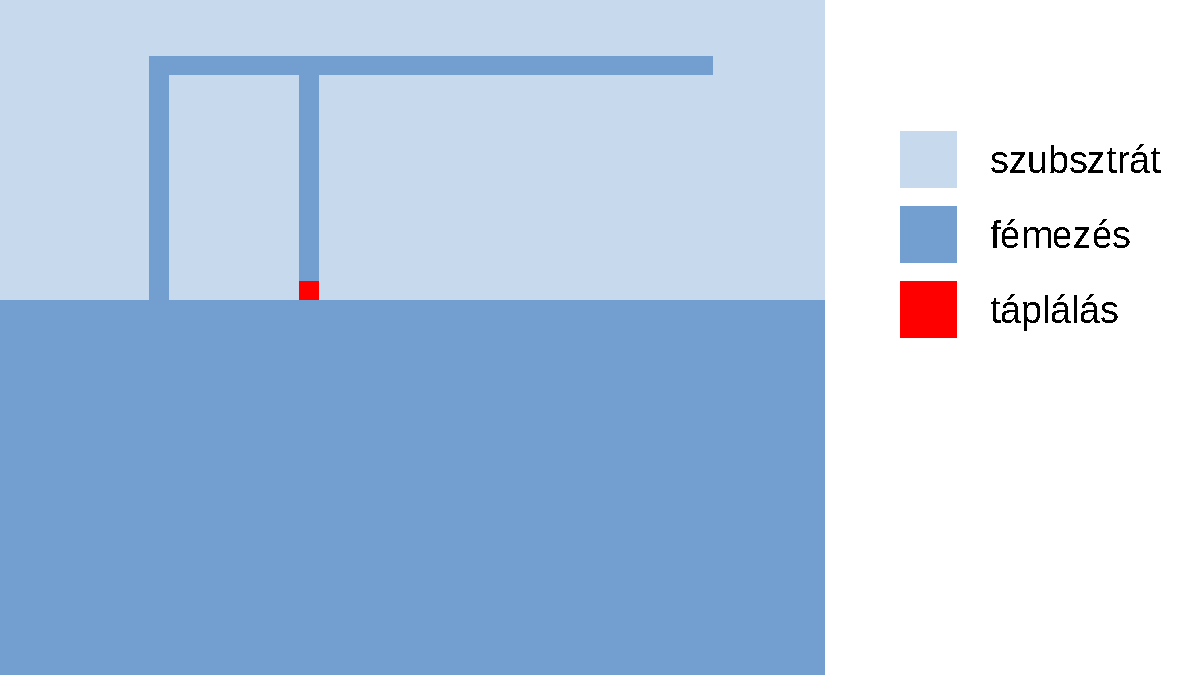
\includegraphics[width=0.6\textwidth]{kep/tipikus_ifa.pdf}
	\caption{Egy tipikus nyomtatott IFA egy nyomtatott áramköri lap szélén.}
	\label{fig:tipikus_ifa}
\end{figure}
\par Az IFA az ILA (Inverted L Antenna) egy variációja (\ref{fig:tipikus_ila}. ábra). Az IFA előnye az ILA-val szemben a megnövekedett abszolút értékű bemeneti impedancia, ami miatt a működési hullámhosszhoz képest kis méretben is jobban használható, könnyebben illeszthető a tápláló hálózathoz. Ezek miatt az IFA-t szélesebb körben alkalmazzák, például mobil eszközökben, ahol az antenna számára rendelkezésre álló hely erősen korlátozott \cite{multi-band}, ekkor bizonyos esetekben a nyomtatott áramköri lapon (NYÁK) kialakított, megfelelő alakú fémezés maga az antenna.
\begin{figure}[h]
	\centering
	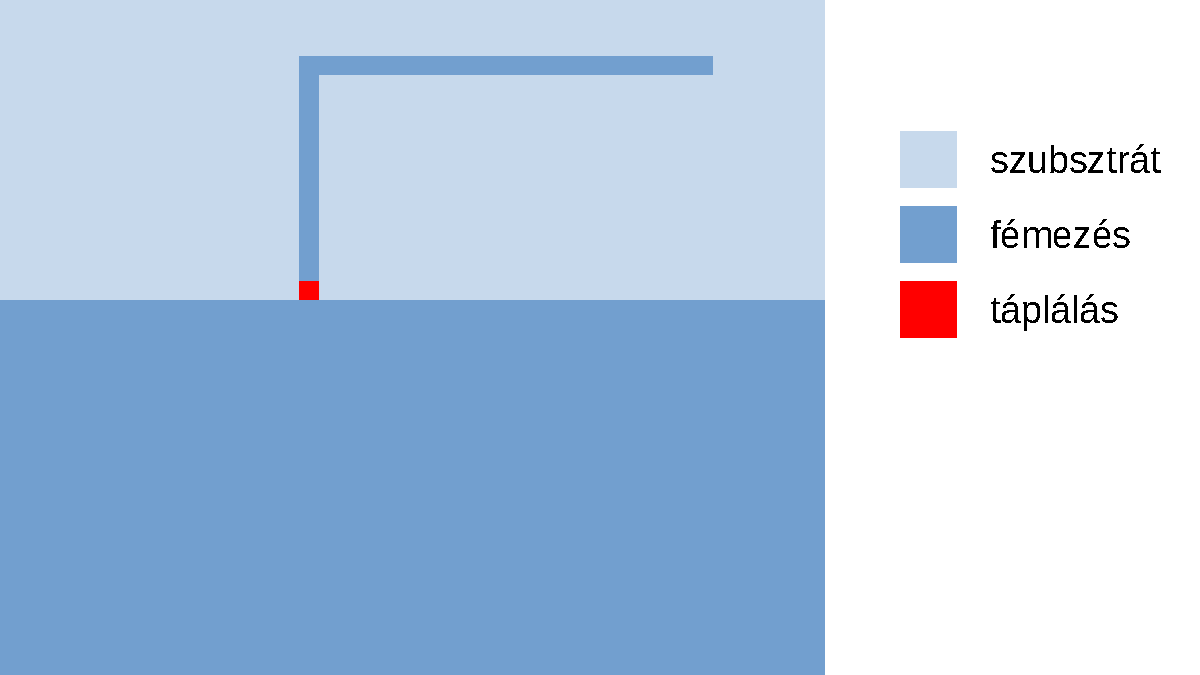
\includegraphics[width=0.6\textwidth]{kep/tipikus_ila.pdf}
	\caption{Egy tipikus ILA egy nyomtatott áramköri lap szélén.}
	\label{fig:tipikus_ila}
\end{figure}
\par A monopól (monopólus) antennákat általában olyankor alkalmazzák, amikor az antenna környezetében egy az antennához képest nagy kiterjedésű vezető található, az ún. alaplap, amit ki lehet használni az antenna sugárzási tulajdonságainak javítására. Ideális esetben az alaplap egy végtelen kiterjedésű és tökéletes elektromos vezető sík. Ekkor a helyettesítő töltések módszerével \cite{fodor} az alaplapot eltávolítva és a monopólt az alaplap síkjára tükrözve egy (a középpontjában a monopóléhoz képest kétszeres feszültséggel gerjesztett) dipól (dipólus) antennát kapunk, amelynek egyik szára az eredeti monopól antenna, ahogy ez \aref{fig:monopol}. ábrán látható.
\begin{figure}[h]
	\centering
	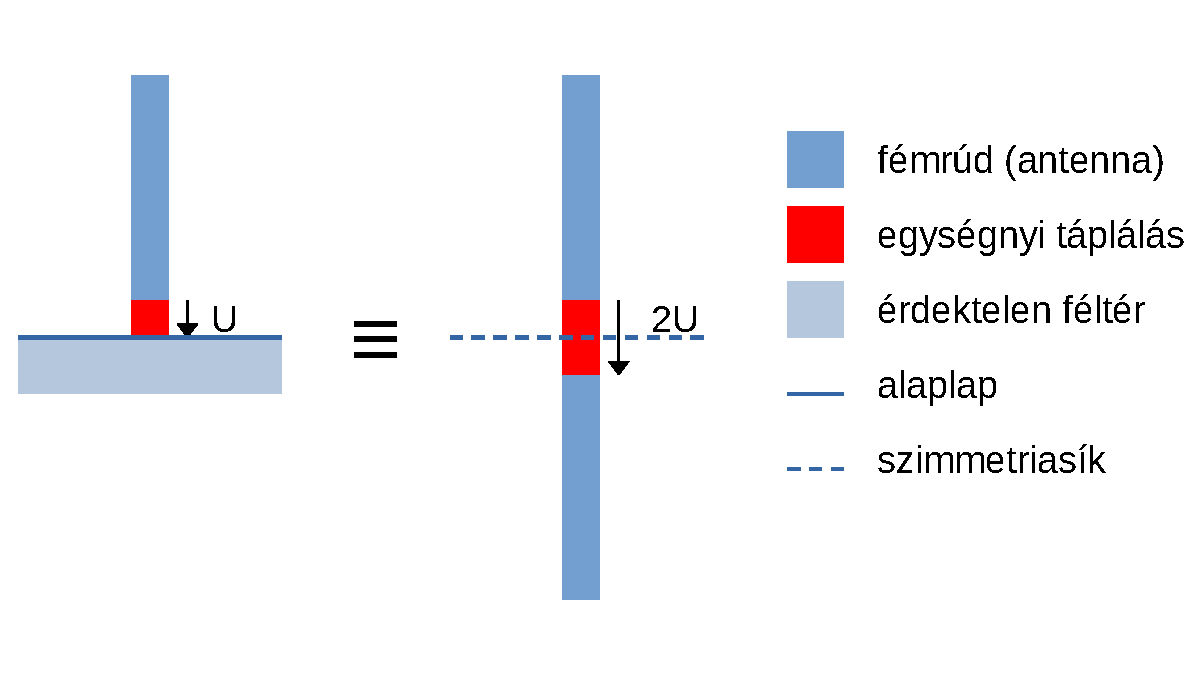
\includegraphics[width=0.6\textwidth]{kep/monopol.pdf}
	\caption{Ideális monopól és ekvivalens dipól.}
	\label{fig:monopol}
\end{figure}
\par Az így kapott antenna az alaplap síkja fölött a monopóluséval megegyező sugárzási karakterisztikát produkál. A monopól esetén az ekvivalens dipól másik szárát az alaplapban indukált áramok hatása helyettesíti, így jön létre a megegyező sugárzási karakterisztika.
\par A fenti helyettesítési módszer nem mindig használható, például egy NYÁK-on kialakított nyomtatott monopól antenna esetén nem, hiszen ekkor legfeljebb a NYÁK földkitöltése tekinthető alaplapnak, de ez messze nem végtelen kiterjedésű, ráadásul az antenna a földkitöltés síkjában helyezkedik el, emiatt nincs értelme a NYÁK síkjára való tükrözésnek. Ehelyett azt a megközelítést érdemes használni a monopól antenna viselkedésének leírásához, ami szerint a nyomtatott antenna és a NYÁK földkiöltése egy erősen aszimmetrikus dipól egy-egy szárának tekinthető \cite{multi-band}.
\par A monopól antennákat használó struktúrák jellemzője, hogy mind az antenna bemeneti impedanciája, mind a sugárzási karakterisztikája érzékeny az alaplap méretének vagy alakjának megváltozására. Ez a jelenség fokozottan jelentkezik akkor, ha az alaplap kis méretű. Ilyen változásokat képes okozni például vezeténélküli mobil eszközöknél, ha a felhasználó a kezébe veszi a készüléket, a fejéhez közel emeli, vagy éppen onnan eltávolítja azt -- mint egy mobiltelefon tipikus használata közben. Az előző példában a felhasználó keze, feje és testének többi része bizonyos keretek között az alaplap kiterjesztésének tekinthető, miszerint azzal, hogy a kezébe veszi a készüléket, többszörösére növeli az alaplap méretét, ami könnyen okozhat jelentős változásokat az antenna működésében. A változás azonban nem feltétlenül jelent romlást. A modern mobiltelefonok tervezésénél úgy veszik figyelembe a felhasználó kezét, fejét, stb., hogy azok közelségükkel ne rontsák, hanem egyenesen javítsák az antenna tulajdonságait, például megnöveljék a nyereségét, lecsökkentsék a Q-ját és közel izotróp sugárzóvá tegyék azt.
\par A monopól antennák fent vázolt tulajdonságát részben orvosolni lehet, ha differenciális antennával váltjuk ki őket, mert az utóbbi csoportba tartozó antennák jellemzően kevésbé érzékenyek az antennához közeli nagyobb vezető tárgyak elhelyezkedésére. Persze ez sem általánosan igaz, a differenciális antennákra is lehet jelentős hatása a környezet változásának, mint például a reflektort használó antennáknál, amelyek jellemzően érzékenyek a reflektor alakjának vagy távolságának változására.
\section{Céges háttér}

